\Chapter{Esperimenti}


\Section{Introduzione}
Sono stati condotti diversi esperimenti, cercando di variare i aspetti della configurazione del modello e del processo di addestramento, al fine di ottimizzare le prestazioni nella segmentazione delle immagini mammografiche. Si è cercato di cambiare gli iperparametri uno alla volta, mantenendo costanti gli altri, per isolare l'impatto di ciascuna modifica. 

\Subsection{Nota sulle Valutazioni}
Nei primi 16 esperimenti, la valutazione sul test set è stata effettuata utilizzando le immagini trasformate, ovvero mantenendo le dimensioni e le modifiche introdotte durante il preprocessing (incluso il resize). A partire dall'esperimento 17, invece, è stata applicata una trasformazione inversa (in particolare il resize inverso) alle ground truth, riportandole alle dimensioni originali. Questo ha permesso una valutazione più corretta e realistica delle performance, evitando possibili distorsioni dovute alle trasformazioni di preprocessing.

\begin{table}[!ht]
    \begin{NiceTabular}{rrX}[rules/color={gray!90},rules/width=1pt]
        \CodeBefore
        \rowcolors{1}{black!5}{}
        \rowcolors{3}{blue!5}{}
        \Body
        \toprule
        \textbf{EXP} & \textbf{Architettura} & \textbf{Parametri Chiave} \\
        \midrule
        1-3 & U-Net 3D & Canali [16,32,64,128] \\
        4-10 & U-Net 3D & Canali [16,32,64,128,256] \\
        12,13 & SliceU-Net 2D & Approccio 2D slice-based \\
        14-21 & U-Net 3D & Varianti profondità/canali \\
        20 & Attention U-Net 3D & Meccanismo di attention \\
        \bottomrule
    \end{NiceTabular}
    \caption{Configurazioni principali dei modelli sperimentali con architetture e parametri chiave.}
    \label{tab:config_modelli}
\end{table}




Lo sviluppo di un sistema di segmentazione automatica efficace richiede non solo un’adeguata progettazione architetturale, ma anche un attento processo di \textbf{ottimizzazione sperimentale}, che tenga conto delle molteplici variabili che influenzano l’apprendimento del modello. In questo capitolo viene descritto in dettaglio il percorso iterativo seguito durante il tirocinio, che ha portato a una progressiva evoluzione del modello fino a raggiungere performance soddisfacenti su immagini MRI 3D della mammella.

\section{Impostazione degli Esperimenti}

Gli esperimenti sono stati condotti in maniera incrementale, seguendo una filosofia di \textbf{ottimizzazione guidata da evidenze}, nella quale ciascuna modifica introdotta agli iperparametri o alla pipeline di preprocessing è stata motivata da osservazioni emerse negli esperimenti precedenti. Tutte le prove sono state documentate e monitorate con precisione.

Per garantire la coerenza e individuare possibili problemi, è stato anche necessario implementare un sistema di \textbf{debugging interno} tramite Python, includendo stampe delle dimensioni dei tensori nei momenti chiave del forward pass e salvataggi intermedi delle immagini durante il training. Questo approccio ha permesso di identificare rapidamente errori legati a mismatch dimensionali, problemi nella gestione della normalizzazione, o trasformazioni incoerenti nei dati di input/output.

\section{Evoluzione Architetturale e Tuning degli Iperparametri}

Il primo esperimento \ref{tab:exp1_config} ha costituito la base di partenza, con una configurazione standard della rete U-Net tridimensionale, con 4 blocchi convoluzionali (\texttt{channels: [16, 32, 64, 128]}), normalizzazione batch, e un resize uniforme applicato a tutte le immagini. Con questa configurazione, è stato ottenuto un \textbf{Dice score} sul test set pari a \textbf{0.7894}.

\begin{table}[H]
	\begin{NiceTabular}{rX}[rules/color={gray!90},rules/width=1pt]
		\CodeBefore
		\rowcolors{1}{black!5}{}
		\rowcolors{3}{blue!5}{}
		\Body
		\toprule
		\textbf{Parametro}      & \textbf{Valore}                                \\
		\midrule
		\textbf{Architettura} & U-Net 3D standard con 4 blocchi convoluzionali \\
		\textbf{Canali} & [16, 32, 64, 128] \\
		\textbf{Normalizzazione} & Batch normalization \\
		\textbf{Resize} & Uniforme su tutte le immagini \\
		\textbf{Dice score (test set)} & 0.7894 \\
		\bottomrule
	\end{NiceTabular}
	\caption{Configurazione del primo esperimento (baseline) con architettura U-Net 3D e risultati ottenuti.}
	\label{tab:exp1_config}
\end{table}


Il passo successivo ha previsto un \textbf{aumento del learning rate} dell’ottimizzatore Adam, passando da \texttt{0.0005} a \texttt{0.005}. Questo semplice cambiamento ha prodotto un incremento della metrica di circa \textbf{+1.17\%}, suggerendo che la rete era in grado di convergere più rapidamente in presenza di un gradiente iniziale più marcato. Da qui è emersa l’intuizione che la rete potesse beneficiare anche di una maggiore profondità: il terzo e il quarto esperimento \ref{tab:exp3-4_results} hanno confermato questa ipotesi, mostrando miglioramenti crescenti in validazione e test con l’introduzione di un ulteriore blocco (\texttt{channels: [16, 32, 64, 128, 256]}), fino a raggiungere \textbf{0.8597} sul test set e \textbf{0.8569} sul validation set.

\begin{table}[H]
    \centering
	\begin{NiceTabular}{rl}[rules/color={gray!90},rules/width=1pt]
		\CodeBefore
		\rowcolors{1}{black!5}{}
		\rowcolors{3}{blue!5}{}
		\Body
		\toprule
		\textbf{Parametro} & \textbf{Valore} \\
		\midrule
		\textbf{Architettura} & U-Net 3D profonda con 5 blocchi convoluzionali \\
		\textbf{Canali} & [16, 32, 64, 128, 256] \\
		\textbf{Normalizzazione} & Batch normalization \\
		\textbf{Dice score (test)} & 0.8597 \\
		\textbf{Dice score (validazione)} & 0.8569 \\
		\bottomrule
	\end{NiceTabular}
	\caption{Risultati degli esperimenti 3-4 con architettura U-Net 3D più profonda. L'aggiunta di un quinto blocco convoluzionale ha portato a significativi miglioramenti nelle metriche.}
	\label{tab:exp3-4_results}
\end{table}

A partire dal quinto esperimento \ref{exp5_comparative} è stata esplorata una \textbf{combinazione di modifiche strutturali}, tra cui il passaggio da \textbf{Adam} ad \textbf{AdamW}, il cambiamento della \textbf{normalizzazione} da \textbf{Batch} a \textbf{Instance} e l’utilizzo di una \textbf{loss} \textbf{composita} (\textbf{Focal} + \textbf{Dice} \textbf{Loss}), ciascuna ponderata per gestire in modo bilanciato gli squilibri tra le classi. Questa configurazione ha prodotto ottimi risultati in validazione (\textbf{0,8623}) e (\textbf{0,8597}) sul test set.
\begin{table}[H]
    \centering
    \begin{NiceTabular}{rl}[rules/color={gray!90},rules/width=1pt]
        \CodeBefore
        \rowcolors{1}{black!5}{}
        \rowcolors{3}{blue!5}{}
        \Body
        \toprule
        \textbf{Componente} & \textbf{Modifica} \\
        \midrule
        \textbf{Ottimizzazione} & Sostituzione Adam → AdamW \\
        \textbf{Normalizzazione} & Batch → Instance \\
        \textbf{Loss function} & Dice → DiceFocal ($\lambda$ =0.7/0.3) \\
        \textbf{Metriche} & $\Delta$ Valid +3.1\%, $\Delta$ Test +0.32\% \\
        \textbf{Risultati} & Valid: 0.8623, Test: 0.8597 \\
        \bottomrule
    \end{NiceTabular}
    \caption{Analisi comparativa delle modifiche introdotte dall'EXP 5. Tutti i cambiamenti hanno contribuito al miglioramento delle performance.}
    \label{tab:exp5_comparative}
\end{table}


Nei successivi esperimenti, si è indagata ulteriormente la sensibilità del modello al \textbf{learning rate}, che era stato inizialmente portato troppo in basso (\texttt{0.0001}). Ripristinando un valore intermedio (\texttt{0.001}), il Dice score sul test è aumentato di oltre il \textbf{3\%}. Parallelamente, l’introduzione di una strategia di \textbf{learning rate scheduling} \ref{fig:learning_rate_scheduling} (LinearWarmupCosineAnnealingLR) ha portato a miglioramenti più modesti ma stabili.

\begin{figure}[H] 
  	\centering 
 	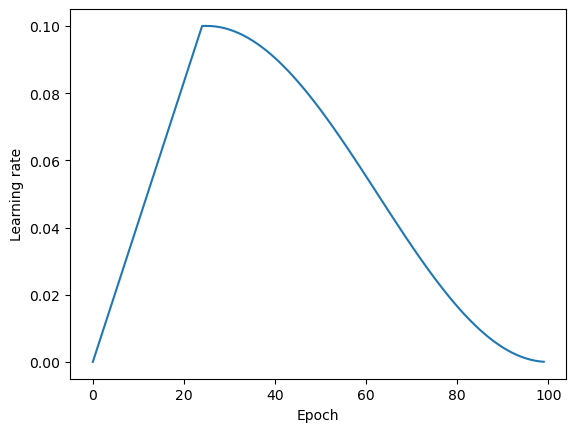
\includegraphics[width=.6\textwidth]{images/2025-07-12-11-28-31.png} 
    \caption{Andamento del learning rate durante il training, con warmup iniziale e successiva discesa coseno.}
    \label{fig:learning_rate_scheduling}
 \end{figure} 



Una seconda linea di sperimentazione ha riguardato il \textbf{trattamento dimensionale} delle immagini. Portando la dimensione da \hlight{384x384} a \hlight{512x512}, si è osservato un ulteriore miglioramento della metrica. Al contrario, strategie basate esclusivamente sul \textbf{padding}, o su un \textbf{mix di resize e padding}, hanno avuto un effetto \textbf{negativo} sulle performance, portando a un crollo significativo della metrica nel nono e decimo esperimento fino a \textbf{0.7576} sul test set e \textbf{0,816} in validazione. 

\begin{table}[H]
    \centering
    \begin{NiceTabular}{rccc}[rules/color={gray!90},rules/width=1pt]
        \CodeBefore
        \rowcolors{1}{black!5}{}
        \rowcolors{3}{blue!5}{}
        \Body
        \toprule
        \textbf{Configurazione} & \textbf{Dimensione} & \textbf{Test Dice} & \textbf{Valid Dice} \\
        \midrule
        \textbf{Baseline} & 384×384 & 0.7894 & 0.7920 \\
        \rowcolor{green!5}
        \textbf{Full Resize} & 512×512 & \textbf{0,8878} & \textbf{0,8934} \\
        \rowcolor{red!5}
        \textbf{Solo Padding} & 512×512 & 0.7576 & 0.8160 \\
        \textbf{Mix Strategie} & Variabile & 0,8857 &  0,8848 \\
        \bottomrule
    \end{NiceTabular}
    \caption{Confronto sistematico degli approcci dimensionali. I valori mostrano come il resize completo produca i migliori risultati, mentre il padding peggiora le performance.}
    \label{tab:dimension_comparison}
\end{table}


\section{Strategia Alternativa: Approccio 2D e Architettura SliceUNet}

In seguito a questi risultati, è stata sperimentata una \textbf{nuova strategia}, volta a esplorare un approccio 2D invece che 3D. Questo ha richiesto l’adozione di una \textbf{ROI size} di tipo \textbf{(512, 512, 1)}, accompagnata da una trasformazione \texttt{RandSpatialCropSamplesd} e da un’opportuna gestione del padding. Per rendere l’intera pipeline compatibile con questo formato, è stata definita un’architettura \textbf{SliceUNet} personalizzata, progettata per operare su singole slice bidimensionali mantenendo il supporto volumetrico per l’aggregazione del risultato finale.

\begin{code}{python}
class SliceUNet(nn.Module):
    def __init__(self, in_channels, out_channels, channels, num_layers):
        super(SliceUNet, self).__init__()
        self.encoder = nn.ModuleList()
        self.decoder = nn.ModuleList()
        self.bottleneck = nn.Conv2d(
            channels[-1], 
            channels[-1], 
            kernel_size=3, 
            padding=1)
        
        for i in range(num_layers):
            self.encoder.append(
                nn.Conv2d(in_channels if i == 0 else channels[i-1], 
                channels[i], 
                kernel_size=3, 
                padding=1)
            )
            self.decoder.append(
                nn.ConvTranspose2d(
                    channels[i], 
                    out_channels if i == num_layers - 1 else channels[i+1], 
                    kernel_size=2, 
                    stride=2)
            )
    
    def forward(self, x):
        enc_features = []
        for layer in self.encoder:
            x = F.relu(layer(x))
            enc_features.append(x)
        
        for layer in self.decoder:
            x = layer(x)
        
        return x
\end{code}



I primi esperimenti con SliceUNet hanno ottenuto risultati interessanti: partendo da \textbf{0.628}, si è passati a \textbf{0.7808}, in test, modificando la strategia di preprocessing da padding a resize. Tuttavia, nonostante l’eleganza e la semplicità computazionale di questo approccio, i risultati non hanno raggiunto i livelli di accuratezza ottenibili con la versione 3D.

\section{Ritorno all’approccio 3D: Affinamento e Validazione}

Per questo motivo, l’attenzione è tornata su modelli tridimensionali, testando configurazioni diverse di \texttt{roi\_size} (ad esempio, \texttt{512x512x16}) e nuove combinazioni architetturali. Esperimenti successivi hanno mostrato che aumentando la profondità lungo l’asse z e spingendo il numero di \textbf{epoche a 150}, si potevano ottenere performance vicine a \textbf{0.8863} in test, che \textbf{costituivano il massimo assoluto fino a quel punto.}

\begin{table}[H]
    \centering
    \begin{NiceTabular}{rccc}[rules/color={gray!90},rules/width=1pt]
        \CodeBefore
        \rowcolors{1}{black!5}{}
        \Body
        \toprule
        \textbf{Tipo} & \textbf{Parametri Chiave} & \textbf{Test Dice} & \textbf{$\Delta$} \\
        \midrule
        \rowcolor{red!3}
        \textbf{2D Base} 
        & SliceUNet, padding, 50 epoche & 0.628 & \color{gray}{-} \\
        \rowcolor{yellow!3}
        \textbf{2D Migliorato} 
        & SliceUNet, resize $512\times512$  & 0.7808 & \color{green!70!black}{\textbf{↑24.3\%}} \\
        \rowcolor{green!8}
        \textbf{3D Intermedio} 
        & U-Net, ROI $512\times512x16$ & 0.8668 & \color{green!70!black}{\textbf{↑38.0\%}} \\
        \rowcolor{blue!8}
        \textbf{3D Ottimale} 
        & +150 epoche, asse z profondo & \cellcolor{blue!10}\textbf{0.8863} & \cellcolor{blue!10}\color{blue!80!black}{\textbf{↑41.1\%}} \\
        \bottomrule
    \end{NiceTabular}
    \caption{Progressione prestazionale con scala cromatica: dal rosso (baseline) al blu (miglior risultato). I $\Delta$ verdi mostrano il miglioramento cumulativo, mentre il blu evidenzia il picco prestazionale (+41.1\% rispetto alla baseline).}
    \label{tab:3d_color_progression}
\end{table}

\Section{Nuovo approccio di Valutazione}
Un aspetto critico che è emerso in questa fase è stato il modo in cui le predizioni venivano valutate. In effetti, l’adozione di tecniche di preprocessing alterava la struttura delle label, rendendo la metrica poco rappresentativa. È stata quindi introdotta una \textbf{pipeline di trasformazioni inverse} nella fase di test, per riportare le predizioni allo spazio originale e confrontarle correttamente con le etichette intonse.

\begin{code}{python}
def inverse_transform(prediction, original_shape):
    # Resize prediction to original shape
    prediction_resized = F.interpolate(prediction.unsqueeze(0), 
                                       size=original_shape, 
                                       mode='nearest').squeeze(0)   
    # Convert to binary mask   
    prediction_mask = (prediction_resized > 0.5).float()
    return prediction_mask
\end{code}

% Con questa nuova metodologia di test, sono stati ripetuti alcuni esperimenti precedenti. Sebbene i risultati apparissero \textbf{lievemente più bassi in termini assoluti}, la loro \textbf{affidabilità era notevolmente superiore}. In questo contesto, nuove architetture come l’\textbf{Attention U-Net} e reti con struttura compressa ma profonda hanno ottenuto risultati significativi, culminando nel ventunesimo esperimento con un Dice score pari a \textbf{0.9124}, il valore più alto registrato sull’intero test set.

Con questa nuova metodologia di test, sono stati ripetuti alcuni esperimenti precedenti, mantenendo invariati l’architettura, la configurazione degli iperparametri e il preprocessing, ma modificando il modo in cui veniva eseguita la valutazione sul test set. L’introduzione delle \textbf{trasformazioni inverse}, ha evidenziato una differenza sostanziale tra le metriche riportate in precedenza e quelle ricalcolate in condizioni più rigorose. Ad esempio, l’esperimento \textbf{16}, che con il metodo di valutazione originale aveva raggiunto un Dice score di \textbf{0.8863}, è stato ripetuto come esperimento \textbf{20}, ottenendo un valore ridotto di \textbf{0.8567}. 

Nonostante questa lieve flessione nei valori assoluti, la nuova metodologia ha reso i confronti tra modelli molto più affidabili. Alcune architetture, che in precedenza sembravano promettenti ma erano in realtà favorite da un confronto distorto, hanno rivelato prestazioni inferiori alle attese. Al contrario, modelli più solidi e coerenti, come l’\textbf{Attention U-Net} testato nell’esperimento \textbf{19}, hanno confermato la loro efficacia anche sotto il nuovo regime di valutazione, raggiungendo un Dice score di \textbf{0.8415} dopo 150 epoche di addestramento.

Il punto culminante di questa fase è stato rappresentato dall’esperimento \textbf{21}, in cui è stata utilizzata una \textbf{U-Net profonda con cinque livelli e stride finale lungo l’asse z pari a 1}. L’input adottava una ROI size tridimensionale pari a $(512, 512, 8)$, e il training è stato prolungato fino a \textbf{200 epoche}. In queste condizioni, il modello ha raggiunto un Dice score pari a \textbf{0.9124}, il valore più alto registrato su tutto il test set. Questo risultato rappresenta non solo il successo di una specifica configurazione, ma anche la validazione dell’intero processo di ottimizzazione, culminato in un modello accurato, robusto e valutato con criteri metodologicamente solidi.

\begin{table}[H]
\centering
\begin{NiceTabular}{rlccc}[rules/color={gray!85},rules/width=0.8pt]
\CodeBefore
\rowcolors{1}{}{gray!3}
\Body
\toprule
\textbf{EXP} & \textbf{Configurazione} & \textbf{Dice} & \textbf{$\Delta$} & \textbf{Note} \\
\midrule
16 & Config. originale & 0.8863 & \color{red}{-3.3\%} & Sovrastima precedente \\
20 & Stessa config. + val. rigorosa & 0.8567 & \color{gray}{0\%} & Benchmark corretto \\
19 & Attention U-Net & 0.8415 & \color{red}{-1.8\%} vs 20 & Robustezza verificata \\
\rowcolor{blue!7}
21 & U-Net avanzato & 0.9124 & \color{teal}{+6.5\% vs 20} & Nuovo state-of-the-art \\
\bottomrule
\end{NiceTabular}
\caption{Analisi dettagliata dei risultati finali. La colonna $\Delta$ mostra: per EXP 16 la sovrastima rispetto alla nuova metodologia, per EXP 19-21 la variazione rispetto al benchmark corretto (EXP 20).}
\label{tab:final_results_detailed}
\end{table}

